\begin{table*}[t]
\caption{Application Characteristics.}
\label{tab:benchmarks}
\centering
\footnotesize % Necessary?
\begin{tabular}{l|l||r||r|r|r|r||r} \hline
 & & {\bf lines of} & \multicolumn{4}{|c||}{\bf \# of constructs in
   the program} & {\bf Total \#} \\ \cline{4-7}
{\bf Benchmark} & {\bf Description} & {\bf code} & filters & pipelines
& splitjoins & feedbackloops & {\bf of filters}
\\
\hline \hline
FIR & 64 tap FIR & 
125 & 5 & 1 & 0 & 0 & 132
\\ \hline
Radar & Radar array front-end\cite{pca} & 
549 & 8 & 3 & 6 & 0 & 52
\\ \hline
Radio & FM Radio with an equalizer & 
525 & 14 & 6 & 4 & 0 & 26
\\ \hline
Sort & 32 element Bitonic Sort & 
419 & 4 & 5 & 6 & 0 & 242
\\  \hline
FFT & 64 element FFT & 
200 & 3 & 3 & 2 & 0 & 24
\\  \hline
Filterbank & 8 channel Filterbank & 
650 & 9 & 3 & 1 & 1 & 51
\\  \hline
GSM & GSM Decoder & 
2261 & 26 & 11 & 7 & 2 & 46
\\ \hline
Vocoder & 28 channel Vocoder~\cite{seneff80}&  
1964 & 55 & 8 & 12 & 1 & 101
\\ \hline
3GPP & 3GPP Radio Access Protocol~\cite{3gpp} &  
1087 & 16 & 10 & 18 & 0 & 48
\\ \hline
\end{tabular}
\end{table*}

\begin{table*}
\caption{Performance Results.}
\label{tab:performance}
\centering
\footnotesize % Necessary?
\begin{tabular}{l||r|r|r|r||r||r} \hline
& \multicolumn{5}{|c||}{\bf 250 MHz Raw processor} & {\bf C on a 2.2 GHz} \\ 
\cline{2-6} 
{\bf Benchmark} & \multicolumn{4}{|c||}{\bf StreamIt on 16 tiles} & {\bf C on a single tile} & {\bf Intel Pentium IV}\\ 
\cline{2-7}
& {\bf Utilization} &
\begin{tabular}{c}\hspace{-5pt} {\bf \# of tiles} \hspace{-5pt}\\
\hspace{-5pt} {\bf used} \hspace{-5pt}
\end{tabular} &    
 {\bf MFLOPS} & 
\begin{tabular}{c}\hspace{-5pt} {\bf Throughput} \hspace{-5pt}\\
\hspace{-5pt} {\bf (per 10$^5$ cycles)} \hspace{-5pt}
\end{tabular} &    
\begin{tabular}{c}\hspace{-5pt} {\bf Throughput} \hspace{-5pt}\\
\hspace{-5pt} {\bf (per 10$^5$ cycles)} \hspace{-5pt}
\end{tabular} &    
\begin{tabular}{c}\hspace{-5pt} {\bf Throughput} \hspace{-5pt}\\
\hspace{-5pt} {\bf (per 10$^5$ cycles)} \hspace{-5pt}
\end{tabular} \\    
\hline \hline
FIR    & 84\% &  14 & 815 &  1188.1  & 293.5 & 445.6 \\ \hline
Radar  & 79\% & 16 & 1,231 &     0.52  & {\it app. too large} & 0.041 \\ \hline
Radio  & 73\% & 16 & 421 &    53.9  & 8.85 & 14.1 \\ \hline
Sort   & 64\% & 16  & N/A &  2,664.4 & 225.6 & 239.4 \\ \hline
FFT    & 42\% & 16  & 182 &  2,141.9 & 468.9 & 448.5  \\ \hline
Filterbank & 
       41\% & 16  &  644 &   256.4  & 8.9 & 7.0   \\ \hline
GSM    & 23\% & 16 & N/A &    80.9  & {\it app. too large} & 7.76 \\ \hline
Vocoder& 17\% & 15  & 118 &     8.74  & {\it app. too large} & 3.35  \\ \hline
3GPP   & 18\% & 16  & 44 &   119.6  & 17.3  & 65.7   \\ \hline
\end{tabular}
\end{table*}

\section{StreamIt Compiler}
\label{sec:compiler}

We  have  implemented  a  fully-functional  StreamIt  compiler  as  an
extension to  the Kopi Java  Compiler, a component of  the open-source
Kopi   Project\cite{kopi}.   The   compiler  performs   a   number  of
stream-specific optimizations, and targets a conventional uniprocessor
machine,  a   networked  cluster  of  workstation,  or   the  MIT  Raw
architecture.   Raw internally consists  of a  grid of  16 independent
processors,  with  fast  statically  scheduled  communication  between
processor tiles\cite{rawshort}.   We have also developed  a library in
Java that  allows StreamIt code to  be executed as  pure Java, thereby
providing a verification mechanism for the output of the compiler.

The compilation process for streaming programs contains many novel
aspects because the basic unit of computation is a stream rather than a
procedure.  In order to compile stream modules separately, we have
developed a runtime interface---analogous to that of a procedure call for
traditional codes---that specifies how one can interact with a black box
of streaming computation.  The stream interface contains separate phases
for initialization and steady-state execution; in the execution phase,
the interface includes a contract for input items, output items, and
possible message production and consumption.

\begin{figure}
  \centering
  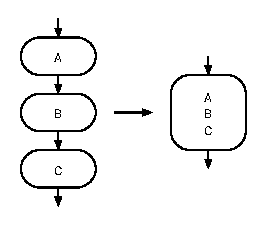
\includegraphics{fusion-vert}
  \caption{Vertical fusion.  Sequential filters in a pipeline are
    joined into a single filter.}
  \label{fig:vert-fusion}
\end{figure}
\begin{figure}
  \centering
  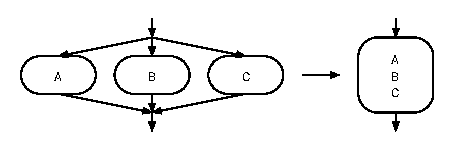
\includegraphics{fusion-horiz}
  \caption{Horizontal fusion.  Parallel filters in a split-join are
    joined into a single filter.}
  \label{fig:horiz-fusion}
\end{figure}

Compiling for Raw involves constructing an expanded stream graph from
the input program, and then partitioning this into 16 sections to fit
on to the tiles of the chip\cite{gordon02}.  The principal technique
for doing this involves \emph{fusing} adjacent filters in the stream
graph to form a single filter.  \emph{Vertical fusion} performs fusion
on successive filters in a pipeline, while \emph{horizontal fusion}
joins the parallel streams in a split-join.  These fusion
optimizations are shown in Figures~\ref{fig:vert-fusion} and
\ref{fig:horiz-fusion} respectively.

The  StreamIt   compiler  also  contains  a   set  of  domain-specific
optimizations for linear  filters, in which each output  is a weighted
sum of  the inputs (e.g.,  FIR, FFT, DCT). The  compiler automatically
detects   linear   filters    and   performs   large-scale   algebraic
simplification   of  adjacent   components,  as   well   as  automated
translation into the frequency  domain when the transformation results
in  faster  code \cite{lamb-pldi03}.  These  techniques yield  average
speedups of 450\% for benchmarks for our evaluation suite.

We have implemented a number of stream programs to test the
performance of our compiler.  These are summarized in
Table~\ref{tab:benchmarks}.  Our benchmarks include several small
kernels which would typically be used as parts of larger applications,
along with some larger systems.

Results of the compiler are given in Table~\ref{tab:performance}.
For each application, we compare the throughput of StreamIt with a
hand-written C program, running the latter on either a single tile of
Raw or on a Pentium IV.  For Radio, GSM, and Vocoder, the C source
code was obtained from a third party; in other cases, we wrote a C
implementation following a reference algorithm.  For each benchmark,
we show MFLOPS (which is N/A for integer applications), processor
utilization (the percentage of time that an {\it occupied tile} is not
blocked on a send or receive), and throughput.  We also show the
performance of the C code, which is not available for C programs that
did not fit onto a single Raw tile (Radar, GSM, and Vocoder).

%For the GSM application, the extensively hand-optimized C version
%incorporates many transformations that rely on a high-level knowledge of
%the algorithm, and StreamIt performs an order of magnitude slower.
%However, this version of the compiler is only a prototype, and is not
%yet intended to compete with hand-coded C.  Our code generation strategy
%currently has many inefficiencies, and in the future we plan to generate
%optimized assembly code by interfacing with a code generator.  We
%believe that stream-conscious optimizations can improve the performance
%by an order of magnitude on uniprocessors; moreover, we have yet to
%consider parallel targets, and this is where we expect to find the most
%pronounced benefits of the abundant parallelism and regular
%communication patterns exposed by StreamIt.
